\subsection{RMN: Corrimiento químico de $^7$Li}

\begin{equation}\label{eq:dli}
    \delta_{i} = \frac{1}{N_i^{\text{Si}}} \sum^{N_i^{\text{Si}}}_{\alpha} \delta_{\text{Key}}(\alpha),
\end{equation}
donde
\begin{equation}\label{eq:dkey}
    \delta_{\text{Key}}(\alpha)=\begin{cases}
    18 \text{ppm} & \text{si } \alpha \text{ es un átomo de Si enlazado}\\
    6 \text{ppm} & \text{si } \alpha \text{ es un átomo de Si aislado} 
    \end{cases}
\end{equation}

\begin{equation}\label{eq:nmr}
    I(x) = \sum_{i} V(x, \delta_{i}, \sigma, \gamma),
\end{equation}

En la Figura \ref{fig:viz} se muestra una celda unidad simplificada en dos
dimensiones con condiciones periódicas de contorno para explicar el modelo
de primeros vecinos de las ecuaciones \ref{eq:dli}, \ref{eq:dkey} y \ref{eq:nmr}
para predecir los resultados del corrimiento químico de RMN para espectros 
del sistema Li-Si. Cada átomo de Li contribuye con un pico Voigt, donde su centro
depende del tipo de átomos de Si (enlazado o aislado) en su primera esfera de 
coordinación. El radio de corte para dicha esfera es igual a 3.4 \AA\ para todas 
las concentraciones, esto puede verse en la RDF parcial de Si-Si en la Figura 
\ref{fig:prdfs}. Por ejemplo, para el átomo de Li $1$ se tiene
\begin{equation}
    \delta_1 = \frac{18 \text{ppm} + 6 \text{ppm}}{2} = 12 \text{ppm},
\end{equation}
donde 18 ppm y 6 ppm vienen del átomo enlazado y del aislado, respectivamente,
que se observa en su primera esfera de cordinación. De la misma manera, para 
el átomo $2$ de Li se tiene 
\begin{equation}
    \delta_2 = \frac{18 \text{ppm} + 18 \text{ppm}}{2} = 18 \text{ppm},
\end{equation}
y para el átomo $3$ de Li
\begin{equation}
    \delta_3 = \frac{6 \text{ppm} + 6 \text{ppm}}{2} = 6 \text{ppm}.
\end{equation}
Luego, la intensidad del espectro generada por estos tres átomos es la suma
de sus contribuciones con picos Voigt centrados en los corrimientos químicos
calculados
\begin{equation}
    I = V_1(12\text{ppm}) + V_2(18\text{ppm}) + V_3(6\text{ppm}) + ...,
\end{equation}
y así puede considrarse el resto de los átomos de Li en la estructura.

\begin{figure}[h!]
    \centering
    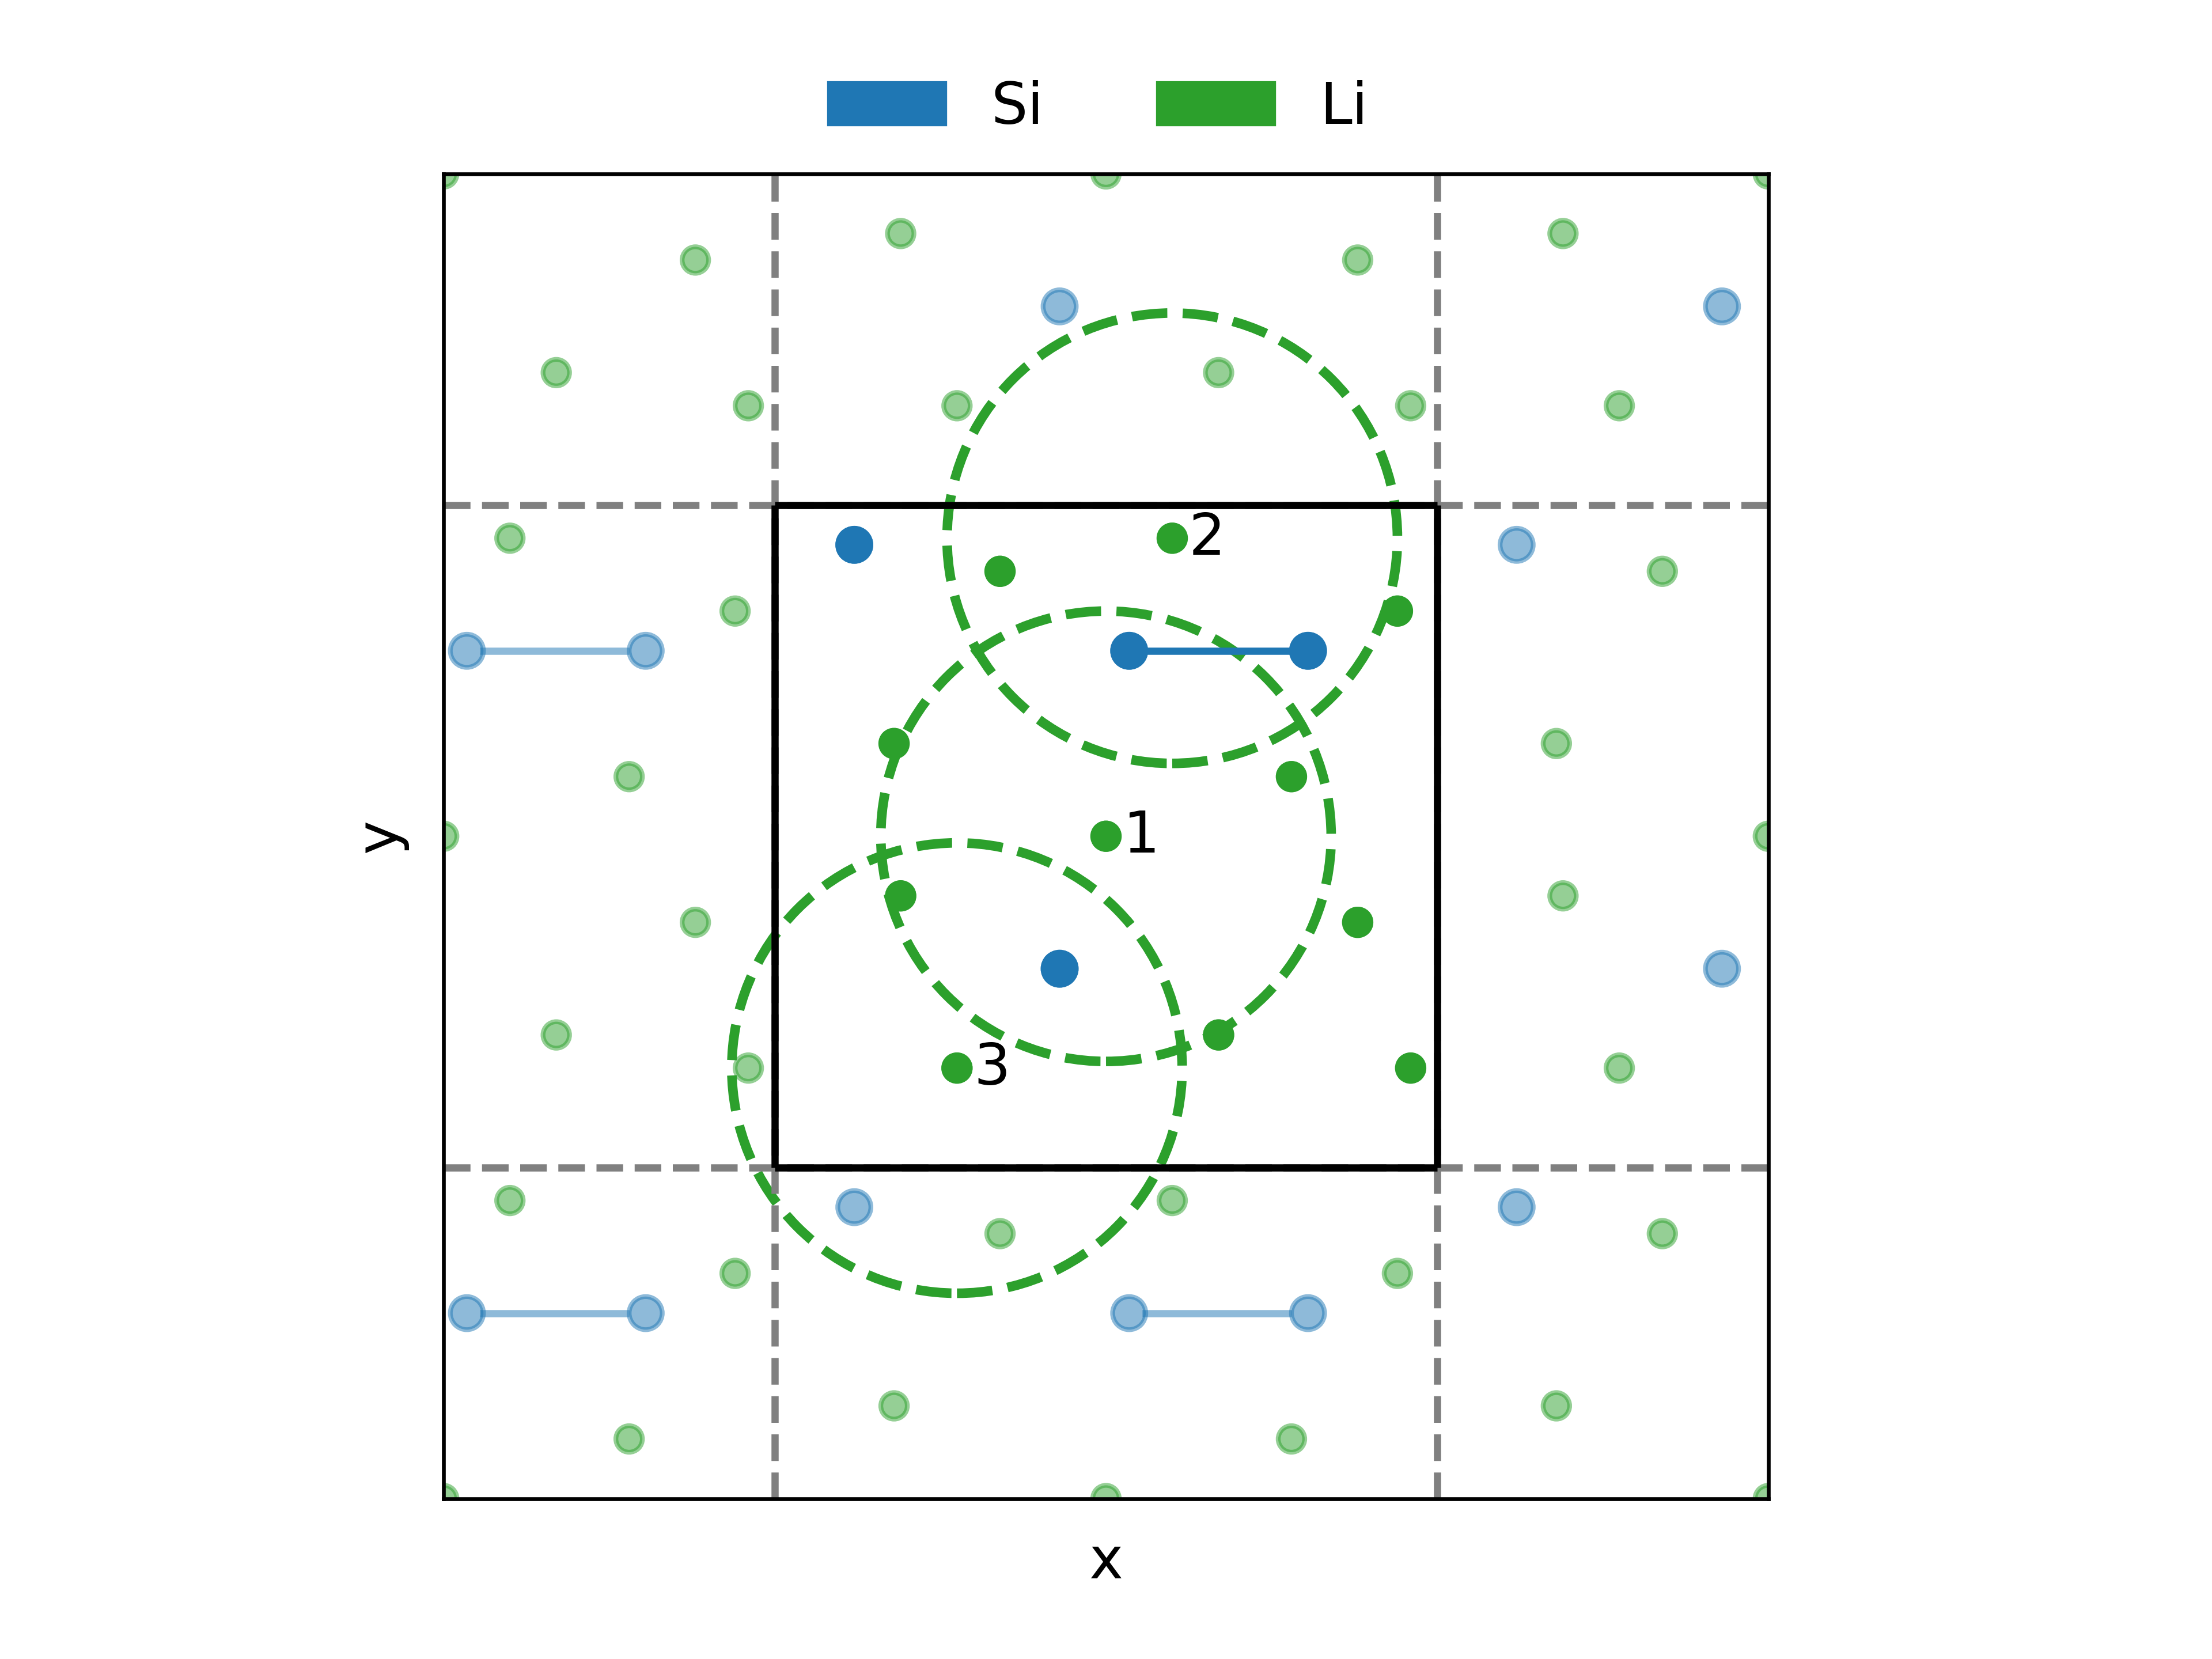
\includegraphics[width=.7\textwidth]{Silicio/prediccion/resultados/nmr/viz.png}
    \caption{Diagrama para explicar el modelo de primeros vecinos que predice los
    espectros de RMN en sistemas Li--Si.} 
    \label{fig:viz}
\end{figure}

\begin{figure}[h!]
    \centering
    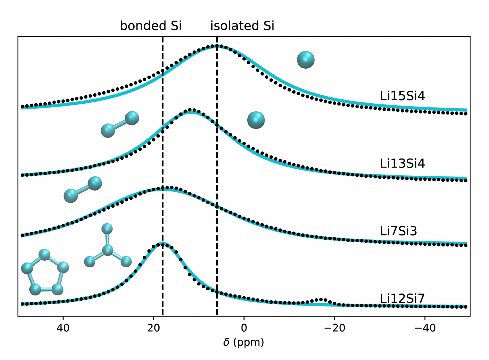
\includegraphics[width=.7\textwidth]{Silicio/prediccion/resultados/nmr/c-nmr.png}
    \caption{Espectros de corrimiento químico de $^7$Li para aleaciones 
    cristalinas. Los puntos corresponden a las mediciones de Key \textit{et al.}
    y las líneas al modelo de primeros vecinos. Las líneas verticales indican las 
    contribuciones del Si enlazado y aislado. Las barras de error son menores que
    el ancho de las líneas.}
    \label{fig:c-nmr}
\end{figure}

\begin{figure}[h!]
    \centering
    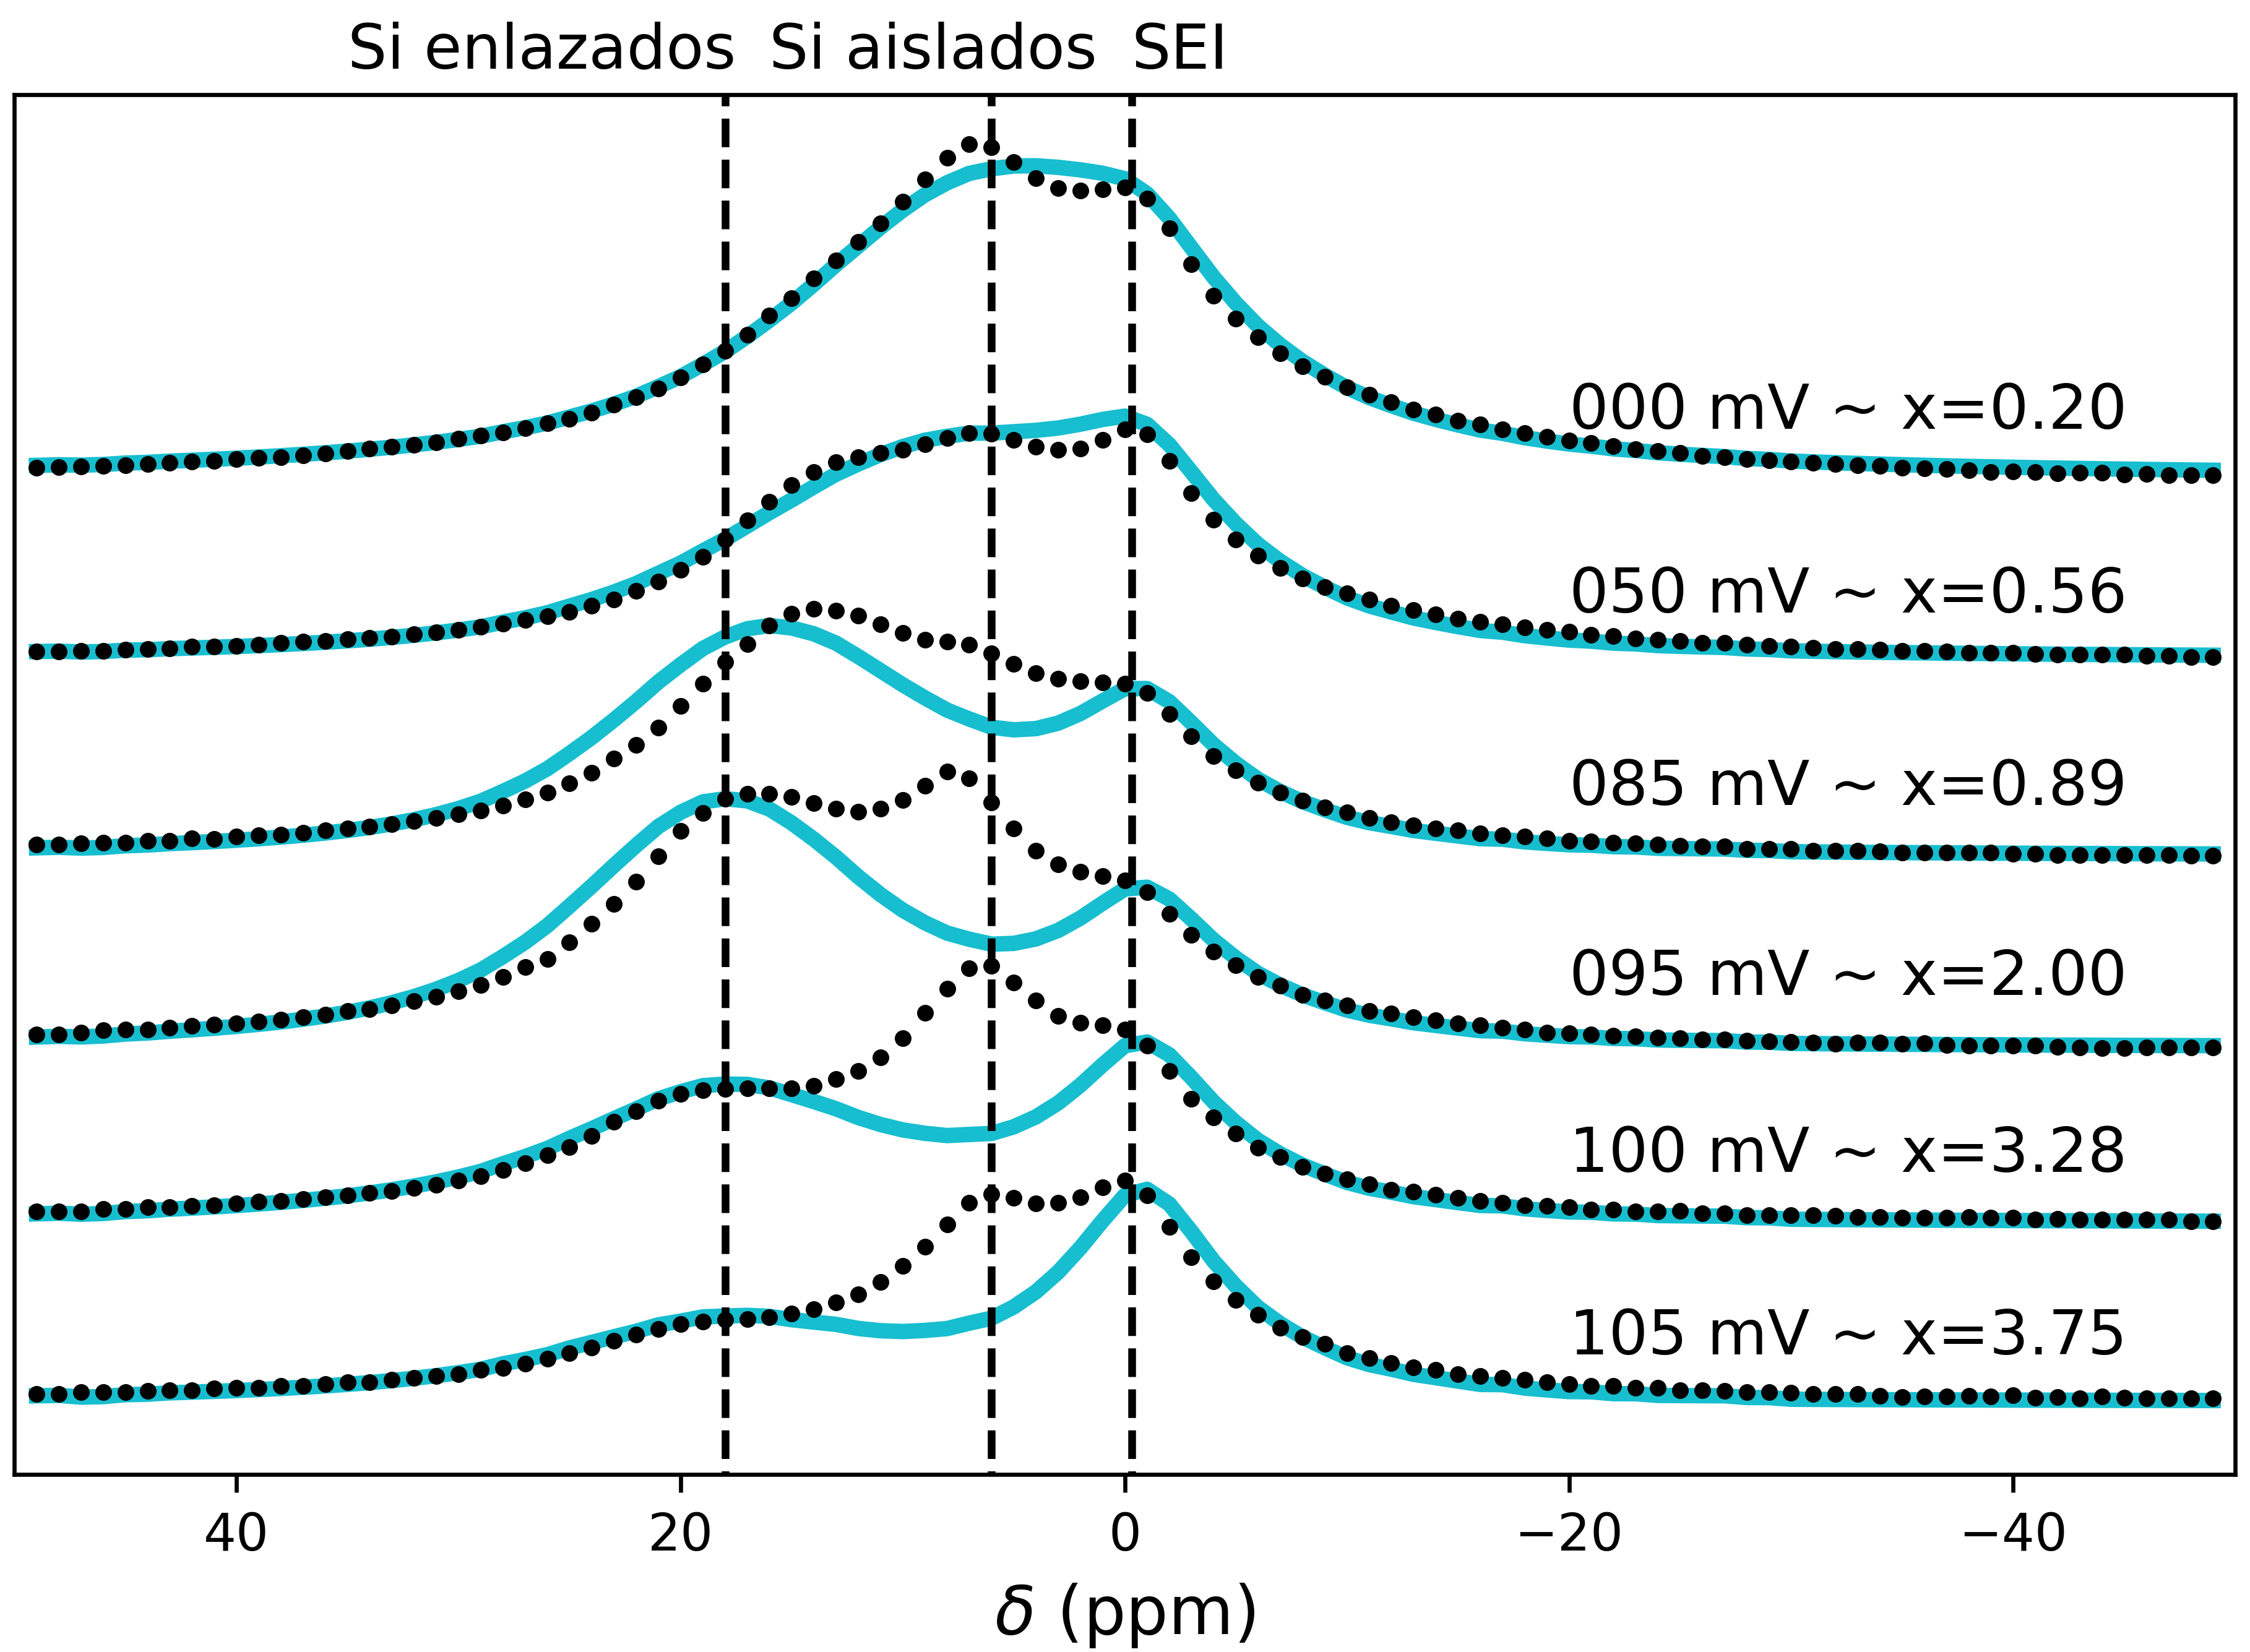
\includegraphics[width=.7\textwidth]{Silicio/prediccion/resultados/nmr/a-nmr.png}
    \caption{Espectros de corrimiento químico de $^7$Li para estructuras amorfas.
    Los puntos corresponden a las mediciones de Key \textit{et al.}. Los 
    resultados del modelo se representan con líneas continuas y se añade una 
    contribución de la SEI para comparar con el experimento. Las líneas verticales 
    indican las contribuciones de la SEI y de los átomos de Si enlazados o 
    aislados. Las barras de error son menores que el ancho de las líneas. Las 
    discrepancias a 6 ppm pueden deberse a una litiación inhomogénea en los 
    experimentos, como se explica en la referencia TODO.} 
    \label{fig:a-nmr}
\end{figure}
